\begin{figure}[t]
\begin{center}
\begin{small}
\begin{sc}
\begin{tabular}{l}
A standard approach based on auxiliary loss func.\\
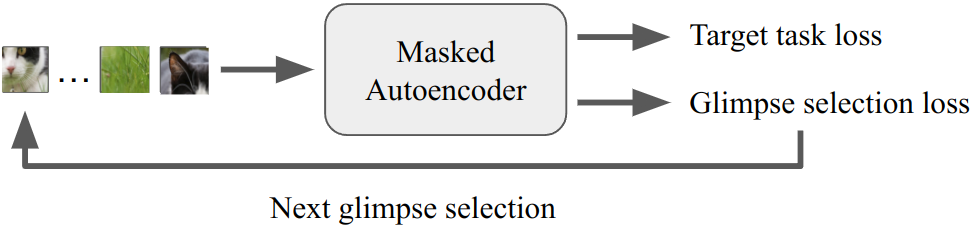
\includegraphics[scale=.23]{fig/teaser/1.png}\\[4pt]
\hline \\[\dimexpr-\normalbaselineskip+4pt]
Our approach based on internal MAE uncertainty\\
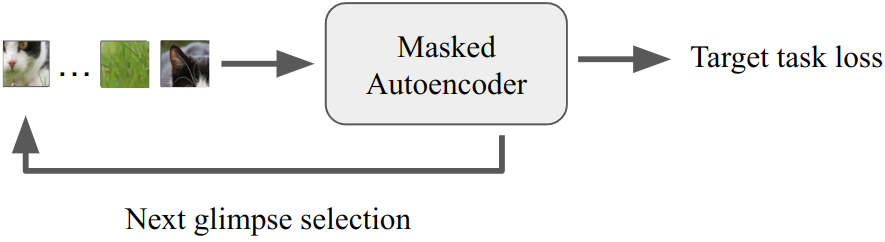
\includegraphics[scale=.23]{fig/teaser/2.png}
\end{tabular}
\end{sc}
\end{small}
\end{center}
\vskip -0.1in
\caption{\textbf{Attention-Map Entropy (AME):} Our approach chooses the most informative observations by reusing the internal uncertainty coded in the attention maps. In contrast to existing methods, it does not require any auxiliary loss functions dedicated to active exploration. Therefore, the training concentrates on the target task loss, not on an auxiliary loss, which improves overall performance.}
\label{fig:teaser}
\end{figure}